\chapter{CONVECCIÓN NATURAL}

Es un mecanismo de transferencia de calor, propio de los medios fluidos y 
considerado como un fenómeno molecular.

\begin{figure}[!h]
\centering
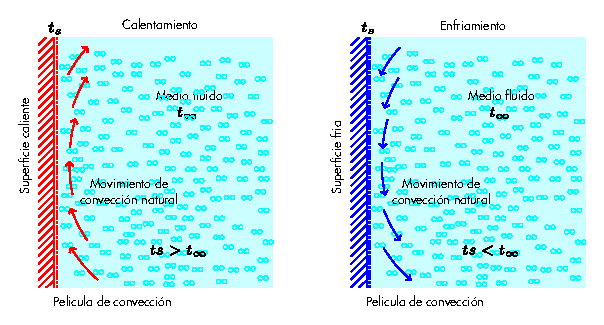
\includegraphics[scale=1.40]{figura04_01.eps}
\end{figure}

Para el calculo del calor transferido se utiliza la ley de enfriamiento de
\emph{Newton}:
\begin{equation*}
    q_c = h\,A\,(t_s-t_\infty)
\end{equation*}

Donde:
\begin{itemize}
    \item $h$: Coeficiente de convección.
    \item $A$: Área de transferencia de calor.
    \item $t_s$: Temperatura de superficie.
    \item $t_\infty$: Temperatura del medio fluido.
\end{itemize}

\begin{equation*}
    q_c \neq 0 \Longrightarrow t_s-t_\infty \neq 0
\end{equation*}
\begin{equation*}
    q_c = 0 \Longrightarrow t_s = t_\infty
\end{equation*}
\begin{equation*}
    q_c \propto h
\end{equation*}

\section{Analogía de la película de convección con una pared}.
\begin{figure}[!h]
\centering
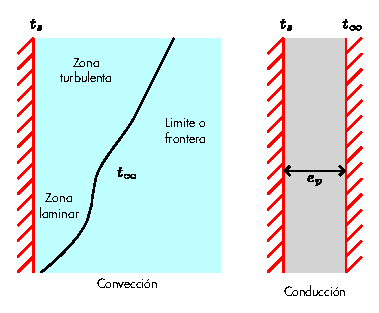
\includegraphics[scale=1.40]{figura04_02.eps}
\end{figure}

Transferencia de calor por conducción:
\begin{equation*}
    q = k\frac{A}{e_p}(t_s-t_\infty)=\frac{t_s-t_\infty}{e_p/k\,A}
\end{equation*}

Resistencia a la conducción:
\begin{equation*}
    R = \frac{e_p}{k\,A}
\end{equation*}

Transferencia de calor por convección:
\begin{equation*}
    q = h\,A(t_s-t_\infty)=\frac{t_s-t_\infty}{1/h\,A}
\end{equation*}

Resistencia a la convección:
\begin{equation*}
    R = \frac{1}{h\,A}
\end{equation*}

Igualando las resistencias:
\begin{equation*}
    \frac{e_p}{k\,A} = \frac{1}{h\,A}
\end{equation*}
\begin{equation*}
    h = \frac{e_p}{k}
\end{equation*}

$e_p$ es un parámetro variable y $k = f(t)$, por tanto:
\textbf{No es posible la analogía}.

\section{Método para la obtención de h}
Existen varios métodos:
\begin{itemize}
    \item Método analítico.
    \item Método empírico.
    \item Método por analogía.
    \item Método o análisis adimensional o análisis por grupos adimensional es.
\end{itemize}

Un \textbf{Grupo adimensional} es la agrupación de dos o mas magnitudes físicas
para obtener un grupo sin dimensiones.

Se consideran dos métodos para el calculo de grupos adimensionales:
\begin{itemize}
    \item Método algebraico.
    \item Método $\Pi$.
\end{itemize}

Una \textbf{magnitud física} es todo ente capaz de ser medido.

Una \textbf{unidad} es la asignación del valor unitario ($1$) a una magnitud
física.

\begin{table}[!h]
\begin{center}
\begin{tabular}{|>{\centering}m{2.4cm}<{\centering}
                |>{\centering}m{1.4cm}<{\centering}
                |>{\centering}m{1.4cm}<{\centering}
                |>{\centering}m{1.4cm}<{\centering}
                |>{\centering}m{1.4cm}<{\centering}
                |>{\centering}m{1.4cm}<{\centering}
                |>{\centering}m{1.4cm}<{\centering}|}
\hline
\textbf{Magnitud} &
\multicolumn{2}{c|}{\textbf{Sistema} \emph{Giorgi}} &
\multicolumn{2}{c|}{\textbf{Sistema técnico}} &
\multicolumn{2}{c|}{\textbf{Sistema ingenieril}} \tabularnewline \hline
&
\textbf{Métrica} &
\textbf{Ingles} &
\textbf{Métrica} &
\textbf{Ingles} &
\textbf{Métrica} &
\textbf{Ingles} \tabularnewline \hline
Masa & $kg$ & $lb$ & $utm$ & $slug$ & $kgm$ & $lbm$ \tabularnewline \hline
Fuerza & $N$ & $lb$ & $kgf$ & $lbf$ & $kgf$ & $lbf$ \tabularnewline \hline
Longitud & $m$ & $pie$ & $m$ & $pie$ & $m$ & $pie$ \tabularnewline \hline
Tiempo & $s$ & $s$ & $s$ & $s$ & $s$ & $s$ \tabularnewline \hline
Temperatura & $K$ & $R$ & $^{\circ}C$ & $^{\circ}F$ & $^{\circ}C$ & $^{\circ}F$
\tabularnewline \hline
\end{tabular}
\caption{Magnitudes en diversas unidades de medición.}
\end{center}
\end{table}

\textbf{\underline{Problema}}: Una esfera maciza se enfría en una corriente
fluida. Encontrar una expresión de grupos adimensionales para hallar de esta
expresión el valor de $h$.

\begin{figure}[!h]
\centering
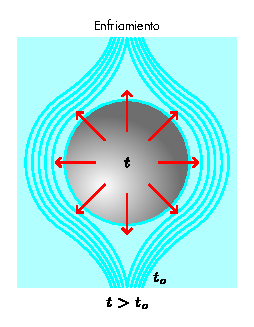
\includegraphics[scale=1.40]{figura04_03.eps}
\end{figure}

\textbf{\underline{Pasos}}:
\begin{enumerate}
    \item Identificación de todas las magnitudes físicas que intervienen en el
        proceso.
        \begin{table}[!h]
        \begin{center}
        \begin{tabular}{|>{\centering}m{4.4cm}<{\centering}
                        |>{\centering}m{5.4cm}<{\centering}|}
        \hline
        \textbf{Esfera} & \textbf{Fluido} \tabularnewline \hline
        \hline
        Diámetro & Velocidad \tabularnewline \hline
        Material & Temperatura \tabularnewline \hline
        Temperatura & Densidad \tabularnewline \hline
        Acabado superficial & Calor especifico \tabularnewline \hline
        & Viscosidad \tabularnewline \hline
        & Coeficiente de conducción \tabularnewline \hline
        \end{tabular}
        \end{center}
        \end{table}
    \item Selección de las magnitudes físicas mas importantes.
        Pueden usarse:
        \begin{itemize}
            \item Analisis experimental.
            \item Analisis de varianza.
        \end{itemize}
        \begin{enumerate}
            \item Diámetro de la esfera ($D$).
            \item Diferencia de temperaturas ($\Delta{t}$).
            \item Velocidad del fluido ($v$).
            \item Densidad ($\rho$).
            \item Viscosidad ($\mu$).
            \item Calor especifico ($C_p$).
            \item Coeficiente de conducción ($k$).
            \item Coeficiente de convección ($h$).
        \end{enumerate}
    \item Expresar las magnitudes físicas elegidas con sus unidades.
        \begin{equation*}
        \def\arraystretch{1.5}
        \begin{array}{@{}cl@{}}
        \toprule
        \text{Magnitud} & \\
        \cmidrule(l){1-2}
        D & [m] \\
        \Delta{t} & [K] \\
        v & [m/s] \\
        \rho & [kg/m^3] \\
        \mu & [kg/m\,s] \\
        C_p & \dfrac{kcal}{kg\,^{\circ}C}
              \dfrac{kgf\,m}{kcal}
              \dfrac{N}{kgf}
              \dfrac{kg\frac{m}{s^2}}{N}
        =\dfrac{kg\,m^2}{kg\,^{\circ}C\,s^2}
        =\left[\dfrac{m^2}{s^2\,K}\right]\\
        k & \dfrac{kcal}{m\,h\,^{\circ}C}
            \dfrac{kg\frac{m^2}{s^2}}{kcal}
        =\dfrac{kg\,m^2}{m\,h\,^{\circ}C\,s^2}
        =\left[\dfrac{kg\,m}{s^3\,K}\right]\\
        h & \dfrac{kcal}{m^2\,h\,^{\circ}C}
            \dfrac{kg\frac{m^2}{s^2}}{kcal}
        =\dfrac{kg\,m^2}{m^2\,h\,^{\circ}C\,s^2}
        =\left[\dfrac{kg}{s^3\,K}\right]\\
        \bottomrule
        \end{array}
        \end{equation*}
\end{enumerate}

\subsection{Método algebraico}
\begin{enumerate}
    \setcounter{enumi}{3}
    \item Aplicar el método algebraico.
        \begin{equation*}
            h = f(D^a,\Delta{t}^b,v^c,\rho^d,\mu^e,C_p^f,k^g)+
                f^{'}(
                    D^{a_1},\Delta{t}^{b_1},v^{c_1},
                    \rho^{d_1},\mu^{e_1},C_p^{f_1},k^{g_1}
                )+
                \cdots
        \end{equation*}
        \begin{equation}
            h = f(D^a,\Delta{t}^b,v^c,\rho^d,\mu^e,C_p^f,k^g)
            \label{algebraico}
        \end{equation}
    \item Reemplazar en cada magnitud de la ecuación sus unidades
        correspondientes.
        \begin{equation*}
            \frac{kg}{s^3\,K} = f\left(
                [m]^a,[K]^b,\left[\frac{m}{s}\right]^c,
                \left[\frac{kg}{m^3}\right]^d,\left[\frac{kg}{m\,s}\right]^e,
                \left[\frac{m^2}{s^2\,K}\right]^f,
                \left[\frac{kg\,m}{s^3\,K}\right]^g\right)
        \end{equation*}
    \item Construir un sistema de ecuaciones lineales para cada exponente.
        \begin{equation}
            \begin{cases}
                [m] & 0 = a + c - 3d - e + 2f + g \\
                [kg] & 1 = d + e +g \\
                [s] & -3 = -c - e - 2f -3g \\
                [K] & -1 = b - f - g \\
            \end{cases}
        \end{equation}
    \item Expresar algunos exponentes en función de otros.
        \begin{equation*}
        \def\arraystretch{1.5}
        \begin{array}{@{}cc@{}}
        \toprule
        \text{Variable} & \text{Frecuencia} \\
        \cmidrule(l){1-2}
        a & 1 \\
        b & 1 \\
        c & 2 \\
        d & 2 \\
        e & 3 \\
        f & 3 \\
        g & 4 \\
        \bottomrule
        \end{array}
        \end{equation*}

        \begin{equation*}
            \begin{split}
            a
                &= -c + 3d + e - 2f - g \\
                &= -(3 - e - 2f - 3g) + 3(1 - e - g) + e - 2f - g \\
                &= -3 + e + 2f + 3g + 3 - 3e - 3g + e - 2f - g \\
                &= -e - g \\
            \end{split}
        \end{equation*}
        \begin{equation*}
            b = f + g - 1
        \end{equation*}
        \begin{equation*}
            c = 3 -e - 2f - 3g
        \end{equation*}
        \begin{equation*}
            d = 1 - e -g
        \end{equation*}
    \item Reemplazar en la ecuación (\ref{algebraico}) y resolver para los
        exponentes.
        \begin{equation*}
            h = f(
                D^{-e-g},
                \Delta{t}^{f+g-1},
                v^{-e-2f-3g+3},
                \rho^{-e-g+1},
                \mu^e,C_p^f,k^g
            )
        \end{equation*}
        \begin{equation*}
            h = f\left(
                \left[\frac{\mu}{D\,v\,\rho}\right]^e,
                \left[\frac{\Delta{t}\,C_p}{v^2}\right]^f,
                \left[\frac{\Delta{t}\,k}{D\,v^3\,\rho}\right]^g,
                \frac{v^3\,\rho}{\Delta{t}}
            \right)
        \end{equation*}
        \begin{equation*}
            \frac{h\,\Delta{t}}{v^3\,\rho} = f\left(
                \left[\frac{\mu}{D\,v\,\rho}\right]^e,
                \left[\frac{\Delta{t}\,C_p}{v^2}\right]^f,
                \left[\frac{\Delta{t}\,k}{D\,v^3\,\rho}\right]^g
            \right)
        \end{equation*}
    \item Verificar.
        \begin{equation*}
            \frac{h\,\Delta{t}}{v^3\,\rho} =
            \dfrac{\left[\frac{kg}{s^3\,K}\right][K]}
            {\left[\frac{m}{s}\right]^3\,\left[\frac{kg}{m^3}\right]} = 1
        \end{equation*}
        \begin{equation*}
            \frac{\mu}{D\,v\,\rho} =
            \dfrac{\left[\frac{kg}{m\,s}\right]}
            {[m]\left[\frac{m}{s}\right]\left[\frac{kg}{m^3}\right]} = 1
        \end{equation*}
        \begin{equation*}
            \frac{\Delta{t}\,C_p}{v^2} =
            \dfrac{[K]\left[\frac{m^2}{s^2\,K}\right]}
            {\left[\frac{m}{s}\right]^2} = 1
        \end{equation*}
        \begin{equation*}
            \frac{\Delta{t}\,k}{D\,v^3\,\rho} =
            \dfrac{[K]\left[\frac{kg\,m}{s^3\,K}\right]}
            {[m]\left[\frac{m}{s}\right]^3\left[\frac{kg}{m^3}\right]} = 1
        \end{equation*}
\end{enumerate}

Quedan por determinar:
\begin{itemize}
    \item Función $f$.
    \item Exponentes $e$, $f$, $g$.
    \item Relación entre grupos adimensionales.
\end{itemize}

Cuya solución se realiza en una fase experimental.

\subsection{Método $\Pi$}
\begin{enumerate}
    \setcounter{enumi}{3}
    \item Aplicar el método $\Pi$.
        \begin{equation}
            f(D,\Delta{t},v,\rho,\mu,C_p,k,h) = 0
            \label{pi}
        \end{equation}
        De estas magnitudes físicas se eligen las mas sencillas y las unidades
        del sistema internacional (SI) se expresan en función de las magnitudes
        elegidas.

        \begin{equation*}
            \begin{cases}
                [m] & D \\
                [kg] & \rho = \left[\frac{kg}{m^3}\right]
                    \rightarrow \rho\,D^3 \\
                [s] & v = \left[\frac{m}{s}\right] \rightarrow \dfrac{D}{v} \\
                [K] & \Delta{t}
            \end{cases}
        \end{equation*}

        \begin{equation*}
            \begin{split}
                N_T 
                    &= \text{\# de magnitudes físicas}
                     - \text{\# de magnitudes elegidas} \\
                    &= 8 - 4 \\
                    &= 4
            \end{split}
        \end{equation*}

        \underline{$\Pi_1$}:\\
        \begin{equation*}
            \mu = \left[\frac{kg}{m\,s}\right]
        \end{equation*}
        \begin{equation*}
            \Pi_1 = \mu\,\frac{m\,s}{kg}
                = \frac{\mu\,D\,\frac{D}{v}}{\rho\,D^3}
                = \frac{\mu}{\rho\,v\,D}
        \end{equation*}

        \underline{$\Pi_2$}:\\
        \begin{equation*}
            C_p = \left[\frac{m^2}{s^2\,K}\right]
        \end{equation*}
        \begin{equation*}
            \Pi_2 = C_p\,\frac{s^2\,K}{m^2}
                = \frac{C_p\,\frac{D^2}{v^2}\,\Delta{t}}{D^2}
                = \frac{C_p\,\Delta{t}}{v^2}
        \end{equation*}

        \underline{$\Pi_3$}:\\
        \begin{equation*}
            k = \left[\frac{kg\,m}{s^3\,K}\right]
        \end{equation*}
        \begin{equation*}
            \Pi_3 = k\,\frac{s^3\,K}{kg\,m}
                = \frac{k\,\frac{D^3}{v^3}\,\Delta{t}}{\rho\,D^3\,D}
                = \frac{k\,\Delta{t}}{\rho\,D\,v^3}
        \end{equation*}

        \underline{$\Pi_4$}:\\
        \begin{equation*}
            h = \left[\frac{kg}{s^3\,K}\right]
        \end{equation*}
        \begin{equation*}
            \Pi_4 = h\frac{s^3\,K}{kg}
            = \frac{h\,\frac{D^3}{v^3}\,\Delta{t}}{\rho\,D^3}
            = \frac{h\,\Delta{t}}{\rho\,v^3}
        \end{equation*}

        La ecuación (\ref{pi}), puede reescribirse como:
        \begin{equation}
            f(\Pi_1,\Pi_2,\Pi_3,\Pi_4) = 0
        \end{equation}
\end{enumerate}

\subsection{Tabla de grupos adimensionales conocidos}
\begin{equation*}
\def\arraystretch{1.5}
\begin{array}{@{}lccc@{}}
\toprule
\text{Nombre} & \text{Símbolo} & \text{Expresión} & \text{Uso} \\
\cmidrule(l){1-4}
\text{Número de \emph{Biot}} & [Bi] &
\dfrac{h}{k}\,L & \text{Conducción} \\
\text{Numero de \emph{Fourier}} & [Fo] &
\dfrac{\alpha}{L^2}\,\theta & \text{Conducción} \\
\text{Número de \emph{Nusselt}} & [Nu] &
h\,\dfrac{D}{k} & \text{Convección natural} \\
\text{Número de \emph{Prandtl}} & [Pr] &
C_p\,\dfrac{\mu}{k} & \text{Convección natural} \\
\text{Número de \emph{Grashof}} & [Gr] &
\left(g\dfrac{D^3}{v^2}\right)(\beta\,\Delta{t}) & \text{Convección natural} \\
\text{Número de \emph{Rayleigh}} & [Ra] &
Pr Gr & \text{Convección forzada} \\
\text{Número de \emph{Reynolds}} & [Re] &
\dfrac{\rho\,v\,D}{\mu} & \text{Convección forzada} \\
\text{Número de \emph{Mach}} & [Ma] & \dfrac{v}{v_s} & \\
\text{Número de \emph{Stanton}} & [St] & & \\
\text{Número de \emph{Péclet}} & [Pe] & & \\
\bottomrule
\end{array}
\end{equation*}

\subsection{Reglas para el manejo de grupos adimensionales}
\begin{itemize}
    \item El producto de dos o mas grupos adimensionales da como resultado otro
        grupo adimensional.
    \item La división entre grupos adimensionales da como resultado otro grupo
        adimensional.
        \begin{equation*}
            \frac{1}{\Pi_1} = \frac{\rho\,v\,D}{\mu} = \text{Re}
        \end{equation*}
        \begin{equation*}
            \frac{\Pi_4}{\Pi_3}
                = \dfrac{\frac{h\,\Delta{t}}{\rho\,v^3}}
                    {\frac{k\,\Delta{t}}{\rho\,D\,v^3}}
                = \frac{h\,D}{k}
                = \text{Nu}
        \end{equation*}
        \begin{equation*}
            \frac{\Pi_2\,\Pi_1}{\Pi_3}
                = \dfrac{\frac{C_p\,\Delta{t}}{v^2}\frac{\mu}{\rho\,v\,D}}
                    {\frac{k\,\Delta{t}}{\rho\,D\,v^3}}
                = \frac{C_p\,\mu}{k}
                = \text{Pr}
        \end{equation*}
\end{itemize}

\section{Ecuaciones recomendadas para $h$}

\textbf{Ecuaciones de \emph{Rice}}:

Si $\text{Gr} > 3$:
\begin{equation}
    \text{Nu}_f = 0.47\,(\text{Gr}_f\,\text{Pr}_f)^{0.25}
    \qquad\text{Tubos horizontales}
\end{equation}
\begin{equation}
    \text{Nu}_f = 0.59\,(\text{Gr}_f\,\text{Pr}_f)^{0.25}
    \qquad\text{Tubos verticales}
\end{equation}

Si $\text{Gr} < 3$: Debe usarse la siguiente gráfica:
\begin{figure}[!h]
\centering
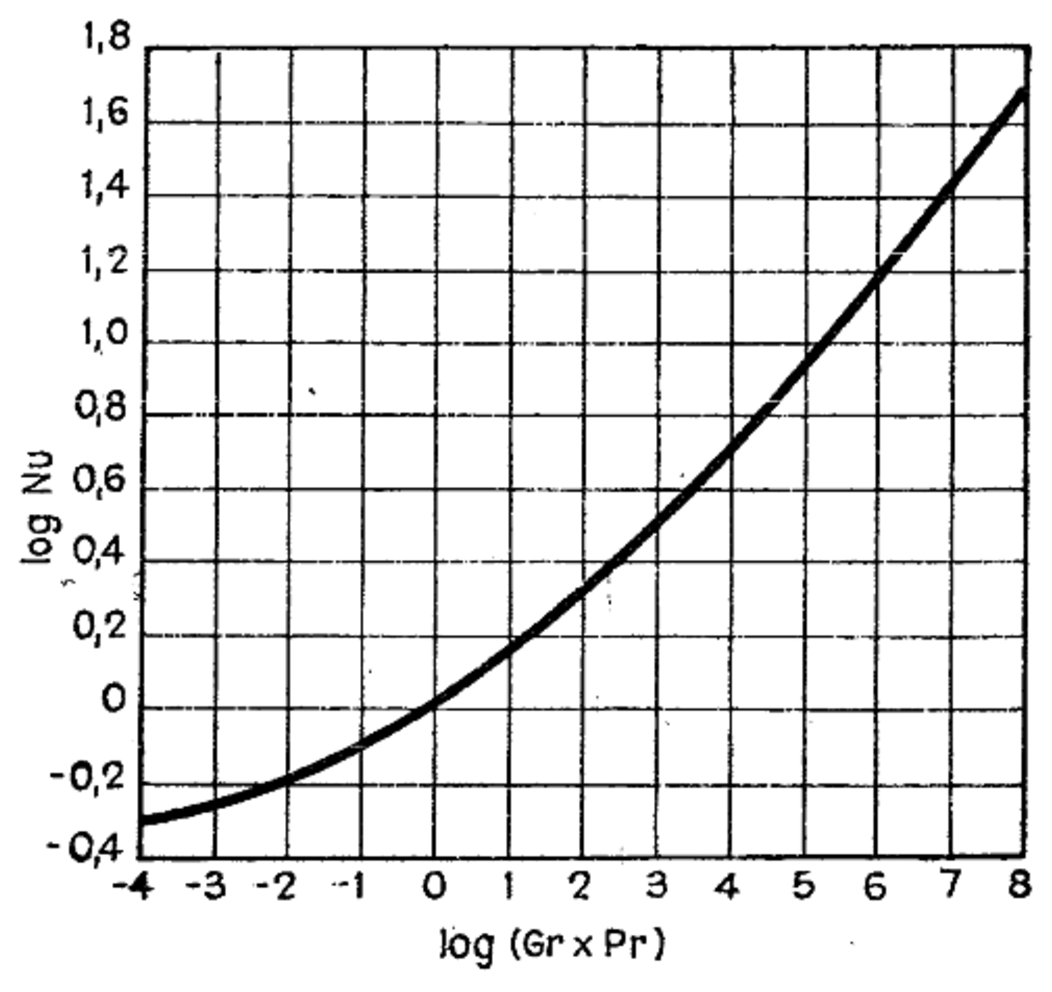
\includegraphics[scale=0.40]{figura04_04.eps}
\end{figure}

El subíndice-índice $f$ (film) refiere a la película de convección natural.

\underline{Propiedades}:\\
\begin{figure}[!h]
\centering
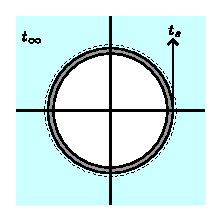
\includegraphics[scale=1.40]{figura04_05.eps}
\end{figure}

\begin{equation}
    \text{Pr} = C_p\,\frac{\mu}{k}
\end{equation}
\begin{equation}
    \text{Gr} = \frac{g\,D^3\,\beta\,\Delta t}{\gamma^2}
\end{equation}
Donde:
\begin{itemize}
    \item $g$: Gravedad local ($9.78 [m/s]$).
    \item $\beta$: Coeficiente de dilatación volumétrico ($[^\circ C^{-1}]$).
    \item $\Delta t$: $t_s - t_\infty$.
    \item $\gamma$: Viscosidad cinemática ($[m^2/s]$).
    \item $D$: Longitud característica.
        \begin{itemize}
            \item Para tubos horizontales: $D=D_E$ (Diámetro externo).
            \item Para tubos verticales: $D=L$ (Altura).
        \end{itemize}
\end{itemize}

\begin{equation}
    \text{Nu} = \frac{h\,D}{k}
\end{equation}
Donde:
\begin{itemize}
    \item $D$: Longitud característica.
        \begin{itemize}
            \item Para ambos tubos: $D=D_E$ (Diámetro externo).
        \end{itemize}
\end{itemize}

\begin{equation}
    t_f (\text{temperatura de película}) = \frac{t_s+t_\infty}{2}
\end{equation}

\subsection{Caso: aire (flujo laminar)}
\begin{figure}[!h]
\centering
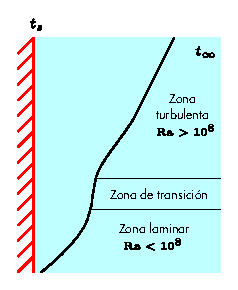
\includegraphics[scale=1.44]{figura04_06.eps}
\end{figure}

\begin{equation}
    h = 2.1\,\Delta t^{0.25}\qquad\text{Paredes horizontales hacia arriba}
\end{equation}
\begin{equation}
    h = 1.1\,\Delta t^{0.25}\qquad\text{Paredes horizontales hacia abajo}
\end{equation}
\begin{equation}
    h = 1.5\,\Delta t^{0.25}\qquad\text{Paredes verticales } L > 0.40
\end{equation}
\begin{equation}
    h = 1.2\,\left(\frac{\Delta t}{L}\right)^{0.25}
    \qquad\text{Paredes verticales } L < 0.40
\end{equation}
\begin{equation}
    h = 1.1\,\left(\frac{\Delta t}{D}\right)^{0.25}
    \qquad\text{Tubos horizontales y verticales}
\end{equation}

\subsection{Caso: Cualquier otro fluido, flujo turbulento, o cualquier forma
geométrica}
\begin{equation}
    \text{Nu} = C\,Ra^a
\end{equation}

Donde:
\begin{itemize}
    \item $C$, $a$, se extraen de la tabla $8-3$ del libro ``Transferencia de
        Calor'', de \emph{Pitts}.
\end{itemize}

\section{Convección en régimen transitorio}
Cuando el medio fluido es demasiado grande, su temperatura ($t_\infty$) no
tiende a permanecer constante, por tanto $h$ y $q_c$ también son constantes.
Esto se denomina ``convección en régimen permanente''.

Cuando el medio tiene su temperatura no constante ($t_\infty = f(\theta)$, tanto
su $h$ como su $q$ son variables. Esto se denomina ``convección en régimen no
permanente'' o ``convección en régimen transitorio''.

\subsection{Deducción de $t = f(\theta)$}
Se debe realizar un balance:

\begin{equation*}
    q_p\,\text{calor perdido por convección natural} = 
    q_s\,\text{calor sensible ganado por el fluido}
\end{equation*}
\begin{equation*}
    -q_c = q_s
\end{equation*}
\begin{equation*}
    -h\,A\,(t_s-t) = m\,C_p\,\frac{dt}{d\theta}
\end{equation*}
\begin{equation*}
    -\frac{dt}{t_s-t_\infty}\,\frac{C_p}{h} = \frac{A}{m}\,d\theta
\end{equation*}
\begin{equation*}
    -\frac{\bar{C_p}}{\bar{h}}\,\int_{t_i}^{t_f}\frac{dt}{t_s-t} =
        \frac{A}{m}\,\int_0^{\theta}\,d\theta
\end{equation*}
\begin{equation*}
    -\frac{\bar{C_p}}{\bar{h}}\,\ln\left(\frac{t_s-f_f}{t_s-t_i}\right) =
        \frac{A}{m}\,\theta
\end{equation*}
\begin{equation}
    \theta =
    -\frac{m\,\bar{C_p}}{A\,\bar{h}}\,\ln\left(\frac{t_s-f_f}{t_s-t_i}\right)
\end{equation}

\subsection{Casos particulares}

Para múltiples tubos horizontales y/o verticales el área total es la suma de las
áreas de cada tubo.

\begin{equation*}
    A_T = N_t A_t
\end{equation*}
\begin{equation*}
    A_t = \pi D_E\,l
\end{equation*}

En placas verticales se debe tomar el volumen por encima de la placa vertical.

\section{Cavidades}
\begin{figure}[!h]
\centering
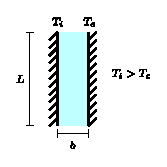
\includegraphics[scale=2.00]{figura04_07.eps}
\end{figure}

\underline{Condición}:
\begin{equation*}
    \frac{L}{b} > 3
\end{equation*}
\\

Se hallan las propiedades del aire a la temperatura promedio:
\begin{equation*}
    \bar{t} = \frac{T_1 + T_2}{2}
\end{equation*}
\\

Y el calculo del número de \emph{Grashof} se hace con el espesor de la cavidad
como longitud característica.
\\
\begin{equation*}
    \text{Gr} = \frac{g\,b^3\,\beta\,(T_1 - T_2)}{\gamma^2}
\end{equation*}

\begin{figure}[!h]
\centering
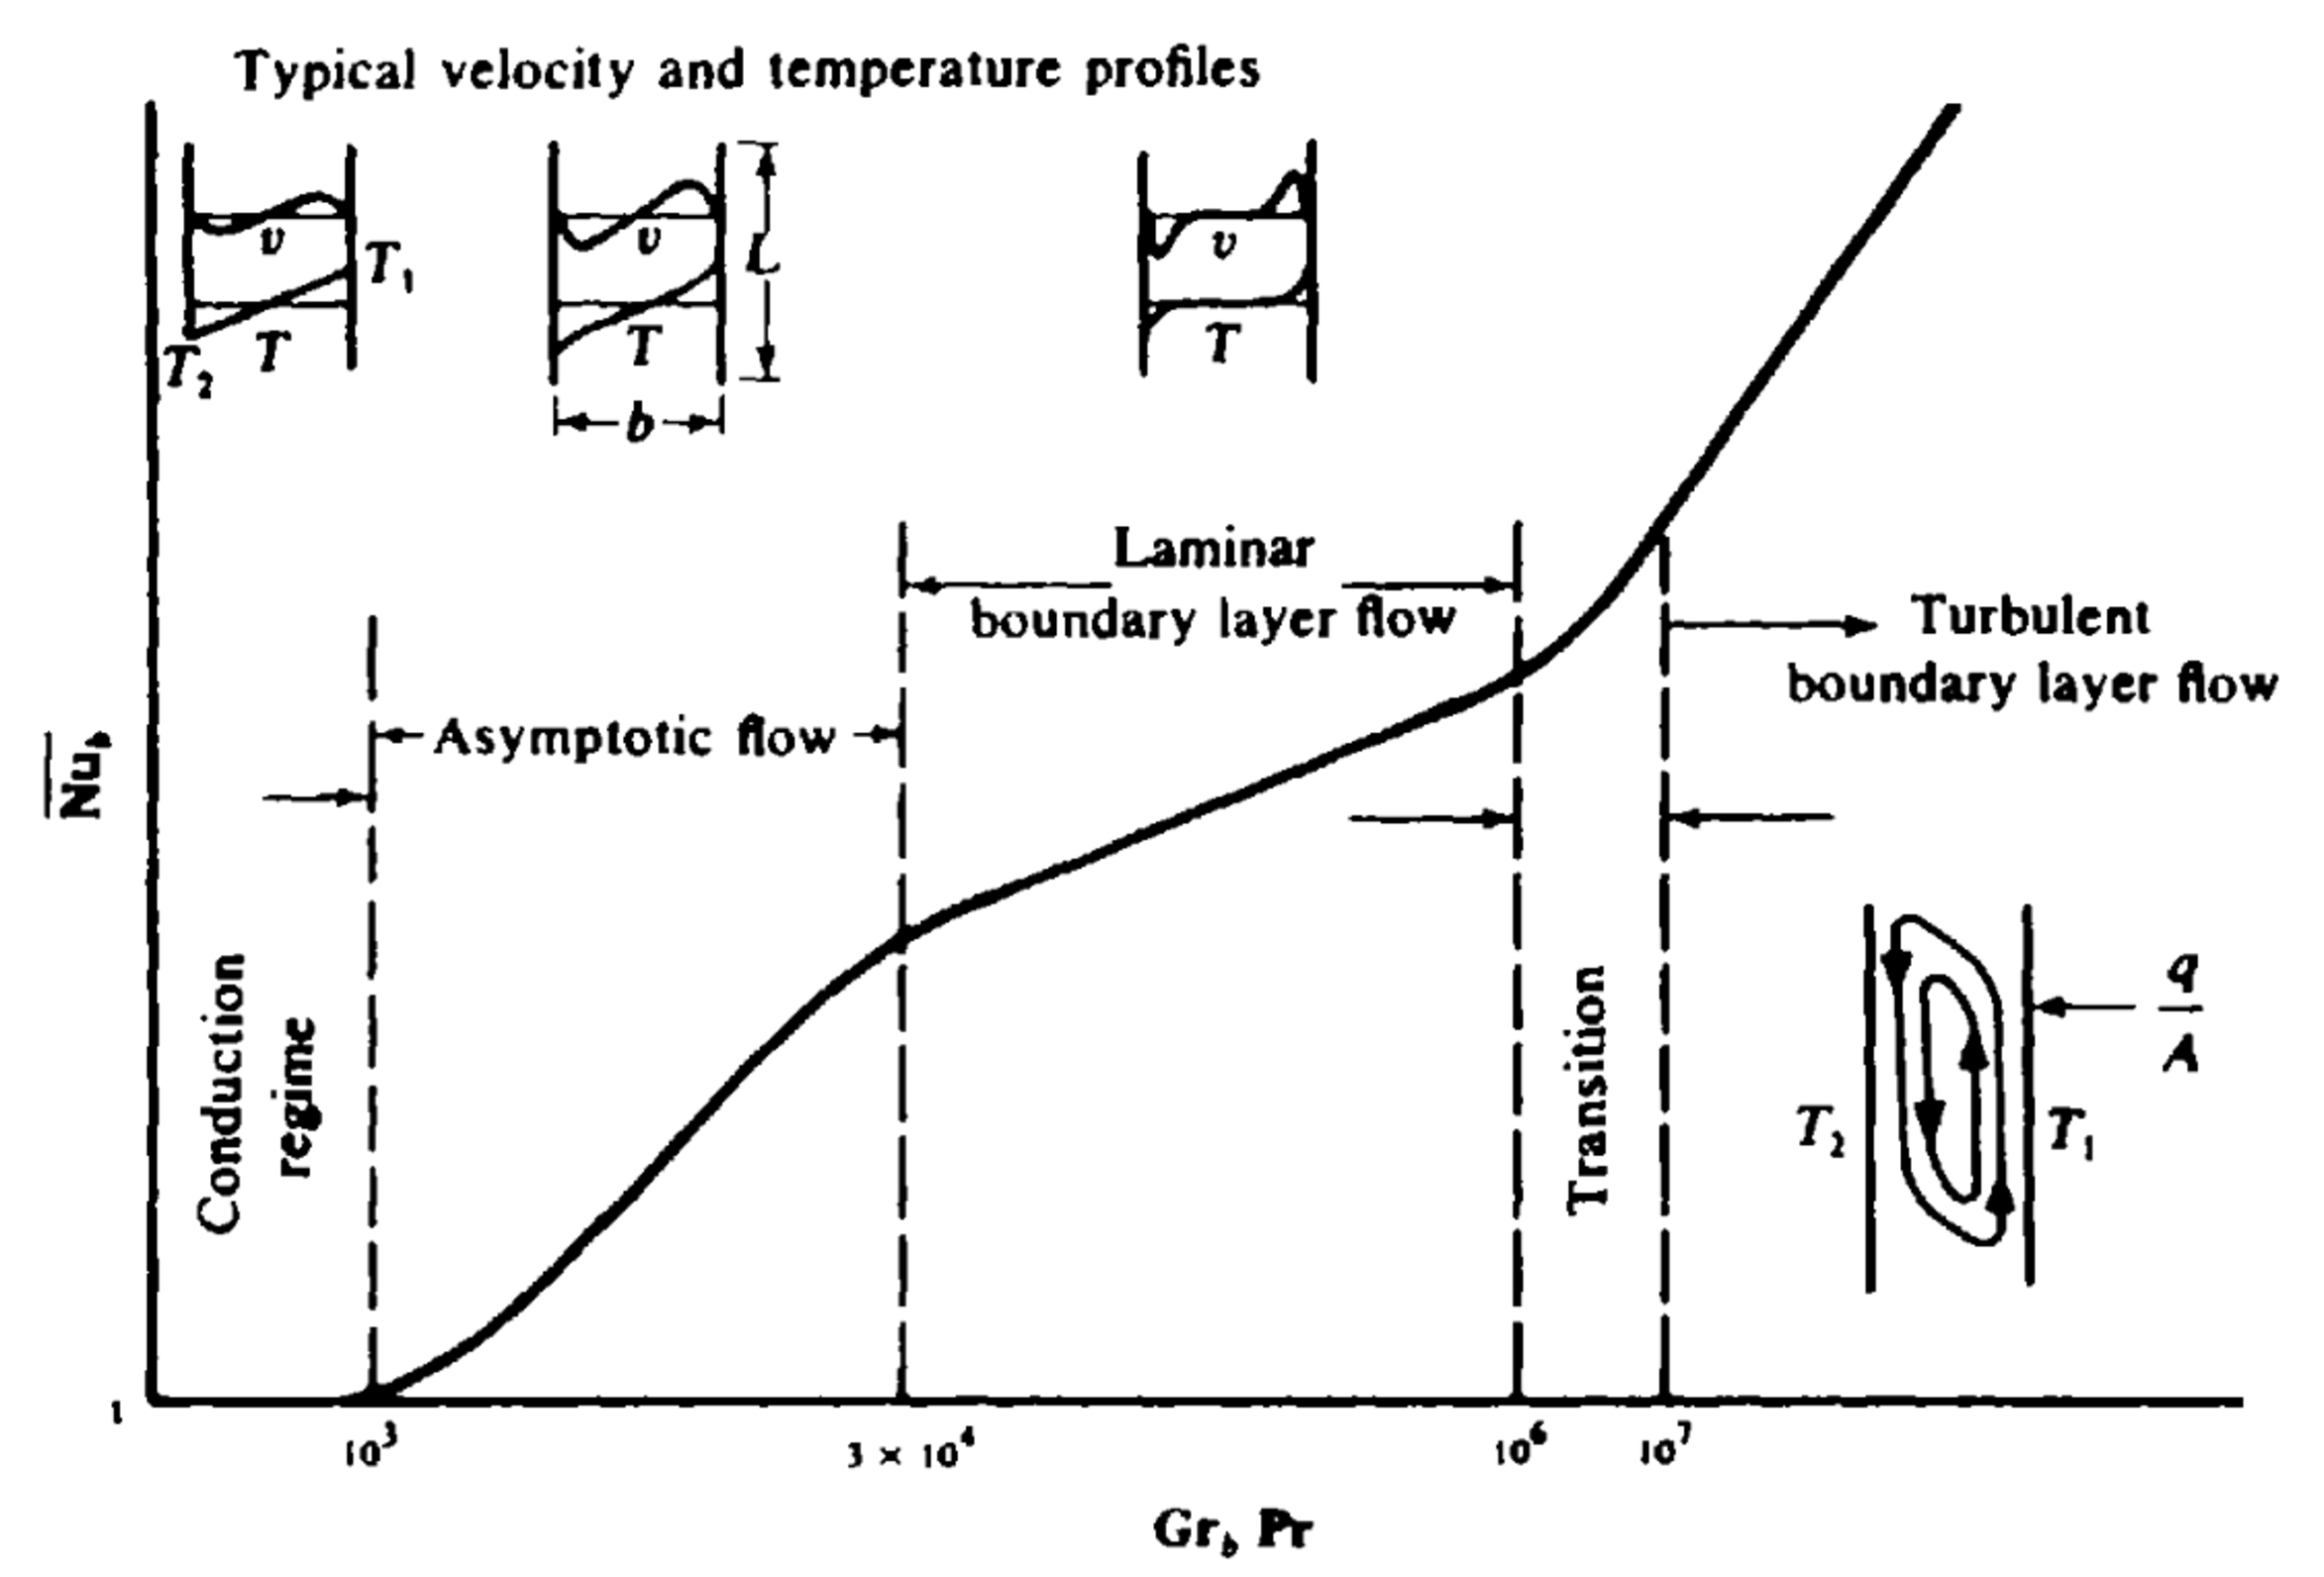
\includegraphics[scale=0.32]{figura04_08.eps}
\end{figure}

Se tienen los siguientes casos:
\begin{table}[!h]
\begin{center}
\begin{tabular}{|>{\centering}m{3.8cm}<{\centering}
                |>{\centering}m{4.4cm}<{\centering}
                |>{\centering}m{4.4cm}<{\centering}|}
\hline
\textbf{Mecanismo} &
\textbf{Condición} &
\tabularnewline \hline
Conducción pura &
$\text{Gr} < 2000$ &
$\text{Nu} = 1$ \tabularnewline \hline
Convección natural en régimen laminar &
$\num{2e4} < \text{Gr} < \num{2e5}$ &
$\text{Nu} = 0.18\,\text{Gr}^{\frac{1}{4}}\,
\left(\frac{L}{b}\right)^{-\frac{1}{9}}$
\tabularnewline \hline
Convección natural en régimen turbulento &
$\num{2e5} < \text{Gr} < \num{2e7}$ &
$\text{Nu} = 0.065\,\text{Gr}^{\frac{1}{3}}\,
\left(\frac{L}{b}\right)^{-\frac{1}{9}}$
\tabularnewline \hline
\end{tabular}
\end{center}
\end{table}

